\section{Sentiment Analyze}

\begin{frame}{Sentiment Analyze}
    
	\begin{block}{Why sentiment analyze?}
		\begin{itemize}
			\item The sentiment of some reviews is different from the actual review scores
			\item Provides merchants with actionable insights for product improvement
		\end{itemize}
	\end{block}
    
	\begin{block}{Steps}
		\begin{itemize}
			\item Model: Pre-trained BERT
			\item Download the pre-trained BERT model, download the data set for local training, and then score the original data for sentiment tendency
		\end{itemize}
	\end{block}

\end{frame}

\begin{frame}{Sentiment-Rating Correlation \& Outlier Detection}
    
	\begin{block}{1. Methodology}
		\scriptsize
		\begin{itemize}
			\item Adjusted sentiment scores to match 5-point rating scale
			\item Computed Sentiment-Rating \textbf{Gap} = \textbf{Rating} - \textbf{Sentiment\_Score\_Scaled}
			\item Detected outliers with |Z| > 2 : 483/10819 ($ \approx ≈ 4.5\%$)
			\item \textbf{General Trend:} Ratings are \textbf{systematically higher} than sentiment scores. 
		\end{itemize}
	\end{block}
    
	\vspace{-20pt}
	\begin{figure}[htbp]
		\centering
		\begin{minipage}[t]{0.50\textwidth}
			\vspace{0pt}
			\centering
			\begin{figure}
				\centering
					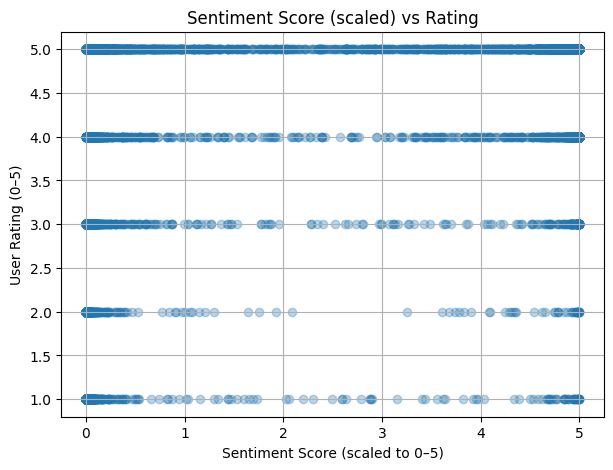
\includegraphics[height=4.5cm]{pic/sentiment_1.png}
			\end{figure}
		\end{minipage}
		\hfill
		\begin{minipage}[t]{0.49\textwidth}
			\vspace{0pt}
			\centering
			\begin{figure}
				\centering
					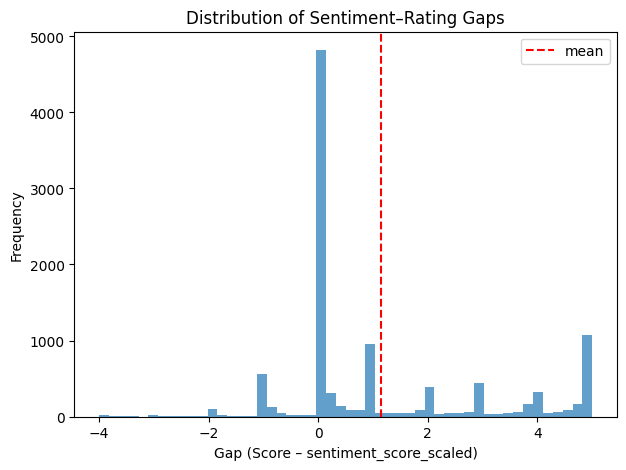
\includegraphics[height=4.5cm]{pic/sentiment_2.png}
			\end{figure}
		\end{minipage}
	\end{figure}

\end{frame}


\begin{frame}{Sentiment-Rating Correlation \& Outlier Detection}
    
	\scriptsize
	\begin{block}{2. Insights: Why Sentiment $\neq$ Rating}
		a. Text–Sentiment Model Bias
		\begin{itemize}
			\item Key words like "unfortunately", "so good", "used to be good" confuse sentiment detection.
			\item Context-dependent irony or comparison not captured by model.
		\end{itemize}

		\vspace{5pt}
		Example of the model bias:\\
		"the product was exactly \textbf{as advertised and fresh. unfortunately} i keep them in a candy dish in the office and they are going fast. we need to reorder to keep up with demand"
		
		\vspace{5pt}
		b. Human Behavior Factors
		\begin{itemize}
			\item Users express disappointment \textbf{politely}, often masking negative emotions.
			\item Positive service experience (e.g. refund) leads to positive feedback despite low product rating.
			\item Social courtesy bias: buyers avoid leaving harsh ratings or comments.
		\end{itemize}

		\vspace{5pt}
		Example of human behavior bias:\\
		"i was very angry about this but jr mushrooms has said they will \textbf{refund} me for the truffles and even let me keep them. so i \textbf{give jr credit for excellent responsiveness} and customer service, although i still feel they should not be labeled black winter truffles"
	\end{block}
    


\end{frame}









